%-------------------------------------------------------------------------------
% LATEX TEMPLATE - CONCEPT-AWARE GEOLOCATION REPORT
%-------------------------------------------------------------------------------

\documentclass{uva-inf-article}
\usepackage[english]{babel}
\usepackage{amsmath, amssymb, amsfonts}
\usepackage{booktabs}
\usepackage{tabularx}
\usepackage{array}
\usepackage{algorithm}
\usepackage{algorithmic}
\usepackage{graphicx}
\usepackage{subcaption}
\usepackage{multirow}
\usepackage{float}
\usepackage{xcolor}
\usepackage{titlesec}

% Reduce top margin on first page
% \newgeometry{top=25mm, bottom=25mm, left=30mm, right=30mm}

\usepackage[style=authoryear-comp]{biblatex}
\addbibresource{references.bib}

% Format for paragraph-level headings (run-in style like NeurIPS)
\titleformat{\paragraph}[runin]{\normalfont\normalsize\bfseries}{\theparagraph}{0em}{}
\titlespacing*{\paragraph}{0pt}{1.0ex plus 0.5ex minus 0.2ex}{1em}

%-------------------------------------------------------------------------------
%	DOCUMENT METADATA
%-------------------------------------------------------------------------------

\title{Concept-Aware Geolocation with Hierarchical Concept Bottleneck Models}

\assignment{Project AI}

\authors{Pradyut Nair}
\uvanetids{15558169}

%\mentor{Nanne van Noord}
\docent{}

%\group{AI Research Group}

\date{\today}

%-------------------------------------------------------------------------------
%	DOCUMENT CONTENT
%-------------------------------------------------------------------------------

\begin{document}
\maketitle
%\restoregeometry

\begingroup
\setlength{\parskip}{0pt}
\setlength{\baselineskip}{0.9\baselineskip}
\tableofcontents
\endgroup
\pagebreak

\begin{abstract}
Image geolocation, the task of predicting geographic coordinates from visual input, remains challenging due to the inherent ambiguity of similar-looking scenes across different regions. While existing approaches achieve reasonable accuracy through end-to-end learning, they operate as black boxes, providing little insight into \textit{why} a particular location is predicted. This work presents a Concept-Aware Geolocation system that learns interpretable semantic concepts as an intermediate representation for location prediction. We propose a three-stage curriculum learning pipeline combining domain-specific contrastive pretraining, hierarchical text-anchored concept learning, and cross-attention-based geolocation. Our architecture enforces a strict concept bottleneck, ensuring all predictions flow through human-interpretable semantic concepts. Experiments on a 43,000-image street view dataset demonstrate that our approach achieves a median error of 126 km on in-distribution data and 350 km on out-of-distribution GeoGuessr images, while providing patch-level attention maps that reveal which visual regions support concept-based predictions.
\end{abstract}

%-------------------------------------------------------------------------------
%	INTRODUCTION
%-------------------------------------------------------------------------------

\section{Introduction}
\label{sec:introduction}

Visual geolocation has emerged as an important capability for applications ranging from autonomous navigation to content verification \parencite{hays2008im2gps}. The fundamental challenge lies in inferring geographic coordinates from images that may contain ambiguous visual patterns \parencite{li2024visual}. A rural road in South Africa may appear similar to one in Australia, while distinctive architectural styles or vegetation can provide strong localization cues.

Early approaches treated geolocation as scene retrieval against geo-tagged databases \parencite{hays2008im2gps}. PlaNet \parencite{weyand2016planet} reformulated this as classification over geographic cells, and subsequent work improved accuracy through hierarchical structures \parencite{muller2018geolocation, seo2018cpl}, culminating in systems like PIGEON \parencite{haas2024pigeon} that achieve expert-level performance on GeoGuessr, an online game where players identify locations from street view imagery.

However, these approaches operate as opaque end-to-end systems providing no insight into their reasoning. This lack of interpretability poses challenges for safety-critical applications where understanding \textit{why} a location was predicted matters. Without explicit semantic reasoning, models may also learn spurious correlations rather than meaningful geographic indicators.

This work develops a concept-aware geolocation system that predicts locations through explicit semantic reasoning. Our approach offers three advantages: predictions flow through a concept bottleneck ensuring inspectable reasoning; explicit concepts enable generalization to novel locations sharing semantic characteristics; and a learned gating mechanism provides interpretable insights into which features rely on concepts versus visual patterns. We make the following contributions:
\begin{enumerate}
    \setlength{\itemsep}{0pt}
    \item A hierarchical concept bottleneck architecture with two levels of semantic abstraction (fine-grained child concepts and coarse parent concepts) and consistency losses enforcing their relationships.
    \item A text-anchored prototype learning approach where concept representations are initialized from CLIP text embeddings and adapted through learnable residuals, maintaining semantic grounding while enabling visual specialization.
    \item A learned gated fusion mechanism where concept embeddings and spatial image information are combined through a learnable gate that controls the contribution of each source per dimension, providing interpretable insights into which geographic features rely on semantic concepts versus spatial patterns.
    \item Geographic cells (geocells) generated through per-country clustering that allocate prediction granularity according to regional data density.
\end{enumerate}

%-------------------------------------------------------------------------------
%	RELATED WORK
%-------------------------------------------------------------------------------

\section{Related Work}
\label{sec:related}

\paragraph{Visual Geolocation.}
Visual geolocation research has evolved from retrieval-based methods \parencite{hays2008im2gps} to classification over geographic partitions. PlaNet \parencite{weyand2016planet} demonstrated that training CNNs to classify images into approximately 26,000 S2 cells \parencite{s2geometry} could achieve reasonable global geolocation. Hierarchical approaches \parencite{muller2018geolocation} improved performance by predicting at multiple spatial scales, while CPlaNet \parencite{seo2018cpl} introduced combinatorial partitioning for finer-grained predictions. More recently, TransLocator \parencite{pramanick2022world} applied transformers to geolocation through scene classification and geographic cell prediction. ISNs \parencite{muller2018geolocation} pioneered the use of individual scene networks that specialize in different geographic regions, enabling more fine-grained predictions. PIGEON \parencite{haas2024pigeon} achieved expert-level performance on GeoGuessr by combining CLIP-based features with sophisticated geocell prediction, demonstrating that vision-language models provide strong foundations for geolocation tasks.

\paragraph{Vision-Language Models for Geolocation.}
CLIP \parencite{radford2021learning} learns aligned vision-language representations through contrastive learning on 400 million image-text pairs, enabling zero-shot transfer to novel visual concepts through natural language descriptions. StreetCLIP \parencite{streetclip2023} fine-tunes CLIP specifically on street view imagery, improving performance on geographically-relevant visual recognition tasks. GeoCLIP \parencite{cepeda2023geoclip} extends this paradigm by training a location encoder alongside CLIP's image encoder, learning joint embeddings where visually similar locations cluster together regardless of their geographic distance. Cross-view approaches \parencite{toker2021satellite_cvpr} have explored matching street-level imagery with overhead satellite views for localization, leveraging the complementary information available from different viewpoints.

\paragraph{Concept Bottleneck Models.}
The concept bottleneck framework \parencite{koh2020concept} addresses neural network interpretability by inserting a layer of human-understandable concepts between input features and final predictions. This design ensures that all model decisions can be traced to specific concept activations, enabling both interpretation and intervention. Early work required manually annotated concept labels, but subsequent extensions have explored concept learning from language supervision \parencite{yang2023language}, post-hoc transformation of pre-trained networks \parencite{yuksekgonul2022posthoc}, and stochastic concept dependencies \parencite{vandenhirtz2024stochastic}. Interactive systems \parencite{chauhan2023interactive} enable human correction of concept predictions to improve downstream accuracy. Most closely related to our work, \cite{jia2025interpretable} propose a concept-aware framework for interpretable geolocalization that aligns images and GPS coordinates through semantic concepts, demonstrating the value of concept-based reasoning for geographic prediction tasks. Our approach differs by introducing hierarchical concepts (child and parent levels), text-anchored prototypes initialized from vision-language embeddings, and a learned gating mechanism that balances concept versus spatial information.

%-------------------------------------------------------------------------------
%	METHODOLOGY
%-------------------------------------------------------------------------------

\section{Methodology}
\label{sec:methodology}

Our approach follows a curriculum learning strategy \parencite{bengio2009curriculum} that progressively builds a concept-aware geolocation system through three training stages. This staged approach allows each component to specialize before being integrated into the complete system, preventing optimization conflicts between different learning objectives.

\begin{figure}[H]
    \centering
    \begin{subfigure}[b]{\textwidth}
        \centering
        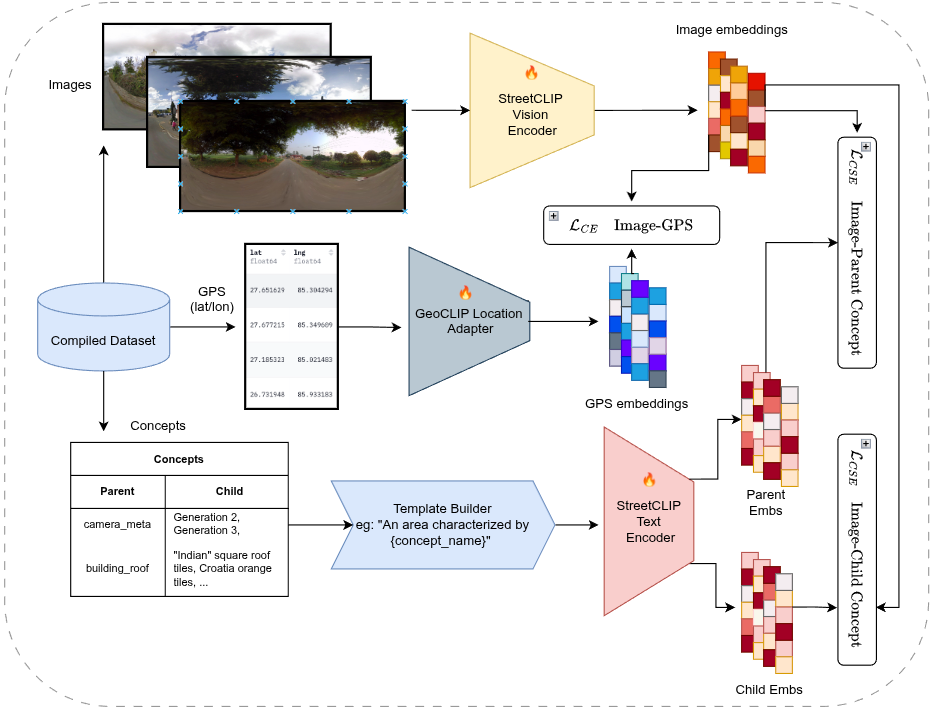
\includegraphics[width=0.85\textwidth]{stage0.png}
        \caption{Stage 0: Domain Contrastive Pretraining}
        \label{fig:stage0}
    \end{subfigure}
    
    \vspace{0.5em}
    
    \begin{subfigure}[b]{\textwidth}
        \centering
        
\includegraphics[width=\textwidth]{stage1_2.png}
        \caption{Stage 1: Concept Learning and Stage 2: Geolocation}
        \label{fig:stage1_2}
    \end{subfigure}
    \caption{Conceptual overview of the three-stage architecture for concept-aware geolocation. \textbf{(a) Stage 0} performs domain contrastive pretraining to align image, GPS, and concept embeddings, with a GPS adapter ($512\text{d} \to 768\text{d}$) projecting GeoCLIP location features to match StreetCLIP image features. \textbf{(b) Stage 1} learns hierarchical concept classification through text-anchored prototypes with cosine similarity. \textbf{Stage 2} predicts geographic coordinates via learned gated fusion: concept embeddings and image embeddings are combined through cross-attention and a cell classification head with offset regression.}
    \label{fig:architecture}
\end{figure}

\subsection{Dataset and Preprocessing}


We train and evaluate our model on a dataset of 43,040 street view panorama images sourced from LearnableMeta \parencite{learnablemeta}, a website that curates challenging GeoGuessr ``metas.'' In the GeoGuessr community, a meta refers to a recurring visual pattern or clue that helps identify a specific country or region. Examples include distinctive road markings, unique vehicle types, characteristic vegetation, or country-specific infrastructure such as bollards, signage styles, or utility poles. Figure~\ref{fig:meta_examples} shows representative examples of such metas. Each sample contains a panoramic street view image, GPS coordinates (latitude and longitude), country name, the meta name, and a ``note'' column describing the meta. The meta name serves as the fine-grained child concept label, capturing scene types such as ``Urban Street'', ``Suburban Road'', and ``Rural Landscape''. The parent concept labels reflect broader categories like ``Urban'', ``Rural'', and ``Natural'', providing a hierarchical semantic structure.

\begin{figure}[H]
    \centering
    \begin{subfigure}[b]{0.32\textwidth}
        \includegraphics[width=\textwidth]{example-image-a}
        \caption{Placeholder: Meta Example 1}
    \end{subfigure}
    \hfill
    \begin{subfigure}[b]{0.32\textwidth}
        \includegraphics[width=\textwidth]{example-image-b}
        \caption{Placeholder: Meta Example 2}
    \end{subfigure}
    \hfill
    \begin{subfigure}[b]{0.32\textwidth}
        \includegraphics[width=\textwidth]{example-image-c}
        \caption{Placeholder: Meta Example 3}
    \end{subfigure}
    \caption{Examples of GeoGuessr metas: distinctive visual patterns that help identify geographic locations. These may include unique road markings, vehicle types, vegetation patterns, or infrastructure elements specific to certain countries or regions.}
    \label{fig:meta_examples}
\end{figure}

The dataset exhibits a hierarchical concept structure with 2,126 child concepts organized under 257 parent concepts. This hierarchy captures semantic relationships: for instance, child concepts ``Urban Street'', ``Commercial District'', and ``Residential Area'' all map to the parent concept ``Urban''. We leverage this hierarchy through consistency losses that encourage predictions at both levels to align.

Data is split into training (70\%), validation (15\%), and test (15\%) sets using stratified sampling by child concept to ensure all concepts appear in training. The same splits are used across all training stages for fair comparison.

\subsection{Geocell Generation}

Traditional approaches partition the Earth's surface uniformly using fixed-resolution grids like S2 cells \parencite{s2geometry}, but this fails to account for non-uniform data distribution. Urban areas contain far more street view imagery than remote regions \parencite{biljecki2021street, wang2025street}. We address this through adaptive per-country clustering that allocates geocells according to regional data density, using only the training split to generate cell centers to prevent data leakage.

For each country with sufficient samples, we convert GPS coordinates to 3D Cartesian positions on the unit sphere and apply K-means clustering with $k = \lceil n / s \rceil$ clusters, where $n$ is the sample count and $s = 500$ is the minimum samples per cell. Countries with fewer samples receive a single cell at their centroid. This process produces 1,048 geocells globally, with dense regions receiving finer granularity than sparse regions. Figure~\ref{fig:geocells} visualizes the resulting tessellation.

\begin{figure}[H]
    \centering
    \begin{subfigure}[b]{0.48\textwidth}
        \includegraphics[width=\textwidth]{geocells_map/geocells_map_finetuned_both.png}
        \caption{Voronoi tessellation of geocells showing cell centers (red markers) and their boundaries. Cell density adapts to regional data availability.}
        \label{fig:geocells_map}
    \end{subfigure}
    \hfill
    \begin{subfigure}[b]{0.48\textwidth}
        \includegraphics[width=\textwidth]{geocells_map/cell_distribution_finetuned_both.png}
        \caption{Distribution of geocells by latitude (left) and hemisphere (right), showing concentration in northern populated regions.}
        \label{fig:geocells_dist}
    \end{subfigure}
    \caption{Adaptive geocell generation through per-country K-means clustering in 3D Cartesian space. The 1,048 geocells provide finer granularity in data-dense regions while maintaining global coverage.}
    \label{fig:geocells}
\end{figure}

\subsection{Stage 0: Domain Contrastive Pretraining}

The first training stage adapts the StreetCLIP vision encoder to our specific domain through multi-objective contrastive learning. While StreetCLIP provides strong geographic priors from pretraining on street view imagery, partial fine-tuning improves downstream concept learning and geolocation accuracy. We unfreeze the top two transformer layers while keeping lower layers frozen to preserve general visual representations.

\paragraph{GPS Adapter.}
The GeoCLIP location encoder produces 512-dimensional GPS embeddings, which we project to 768 dimensions to match the StreetCLIP image feature space for contrastive learning.

\paragraph{Concept Bottleneck Projection.}
A concept bottleneck projects image features to a 512-dimensional embedding space for concept learning:
\begin{equation}
z = \text{ConceptBottleneck}(x) = \text{LayerNorm}(\text{MLP}(\text{LayerNorm}(\text{MLP}(x))))
\end{equation}
where $x \in \mathbb{R}^{768}$ is the image feature and $z \in \mathbb{R}^{512}$ is the concept embedding.

\paragraph{Prototype Projection.}
Text prototypes encoded by the frozen StreetCLIP text encoder (768-dimensional) are projected to the concept embedding space:
\begin{equation}
T_{\text{projected}} = \text{normalize}(W_T \cdot T_{\text{text}})
\end{equation}
where $W_T \in \mathbb{R}^{512 \times 768}$ is a learnable projection matrix.

\paragraph{Alignment Objectives.}
The core alignment objective uses InfoNCE loss \parencite{oord2018infonce} to bring image embeddings closer to their corresponding GPS embeddings while pushing apart embeddings from different locations:
\begin{equation}
\mathcal{L}_{\text{GPS}} = -\frac{1}{B}\sum_{i=1}^{B}\log\frac{\exp(\text{sim}(x_i, g_i)/\tau)}{\sum_{j=1}^{B}\exp(\text{sim}(x_i, g_j)/\tau)}
\end{equation}
where $x_i$ is the L2-normalized image embedding, $g_i$ is the GPS embedding projected to 768 dimensions via the GPS adapter, and $\tau = 0.07$ is the temperature parameter.

Concept alignment losses similarly encourage concept embeddings to cluster according to their semantic labels:
\begin{align}
\mathcal{L}_{\text{child}} &= \text{InfoNCE}(z, T_{\text{child}}, c_{\text{child}}, \tau) \\
\mathcal{L}_{\text{parent}} &= \text{InfoNCE}(z, T_{\text{parent}}, c_{\text{parent}}, \tau)
\end{align}
where $z$ is the L2-normalized concept embedding, $T_{\text{child}}$ and $T_{\text{parent}}$ are text-encoded prototype matrices projected to 512 dimensions, and $c_{\text{child}}$, $c_{\text{parent}}$ are the ground truth concept indices.

Several optional losses provide additional regularization. The hierarchy consistency loss $\mathcal{L}_{\text{hierarchy}}$ uses supervised contrastive learning to encourage embeddings from the same parent category to cluster together in concept space, enforcing semantic relationships between child and parent concepts. The anchor loss $\mathcal{L}_{\text{anchor}} = \text{MSE}(f_\theta(x), f_{\text{vanilla}}(x))$ prevents catastrophic forgetting by penalizing large deviations from frozen vanilla StreetCLIP features $f_{\text{vanilla}}$. The patch-level GPS alignment loss $\mathcal{L}_{\text{patch-GPS}}$ applies contrastive learning between pooled patch embeddings and GPS embeddings, providing spatial regularization at the patch level.

In practice, we find that the core GPS, child concept, and parent concept alignment objectives are sufficient for effective domain adaptation. The hierarchy consistency and patch-GPS losses are optional and were not used in training the final model reported in our experiments ($\lambda_{\text{hierarchy}} = 0$, $\lambda_{\text{patch}} = 0$). The total Stage 0 loss combines these objectives with learned weights and is given by the following equation:
\begin{equation}
\mathcal{L}_0 = \lambda_{\text{GPS}}\mathcal{L}_{\text{GPS}} + \lambda_{\text{child}}\mathcal{L}_{\text{child}} + \lambda_{\text{parent}}\mathcal{L}_{\text{parent}} + \lambda_{\text{hierarchy}}\mathcal{L}_{\text{hierarchy}} + \lambda_{\text{patch}}\mathcal{L}_{\text{patch-GPS}}
\end{equation}

Stage 0 trains for 20 epochs with batch size 128, using differential learning rates: $3 \times 10^{-5}$ for unfrozen encoder layers and $1 \times 10^{-4}$ for projection heads.

\subsection{Stage 1: Text-Prototype Concept Learning}

The second stage learns concept representations through text-anchored classification with hierarchical supervision. The image encoder is frozen to preserve domain alignment from Stage 0, focusing learning on the concept bottleneck.

\paragraph{Text-Anchored Prototypes.}
A key design choice in Stage 1 is how to represent concept prototypes. Rather than learning prototypes from scratch (which risks losing semantic meaning), we initialize them from frozen StreetCLIP text embeddings of concept descriptions. This provides strong semantic grounding: the prototype for ``Urban Street'' begins close to StreetCLIP's representation of that phrase. Learnable residual vectors then allow adaptation to visual patterns specific to our domain while preserving the original semantic structure:
\begin{equation}
T = \text{normalize}(W_T \cdot (T^{\text{base}} + \Delta))
\end{equation}
where $T^{\text{base}} \in \mathbb{R}^{k \times 768}$ contains frozen text embeddings, $\Delta \in \mathbb{R}^{k \times 768}$ is a learnable residual initialized from $\mathcal{N}(0, 0.01)$, and $W_T \in \mathbb{R}^{512 \times 768}$ maps to our 512-dimensional concept embedding space. The final prototypes are L2-normalized.

\paragraph{Cosine Similarity Classification.}
Concept predictions are computed through cosine similarity to prototypes, with learnable temperature scales and per-class bias terms:
\begin{align}
\text{logits}_{\text{child}} &= s_{\text{child}} \cdot (\hat{z} \cdot T_{\text{child}}^T) + b_{\text{child}} \\
\text{logits}_{\text{parent}} &= s_{\text{parent}} \cdot (\hat{z} \cdot T_{\text{parent}}^T) + b_{\text{parent}}
\end{align}
where $\hat{z} = \text{normalize}(z)$ is the L2-normalized concept embedding, $s_{\text{child}}$ and $s_{\text{parent}}$ are learnable logit scales (initialized to 14.0, clamped to 20), and $b_{\text{child}}, b_{\text{parent}} \in \mathbb{R}^k$ are per-class bias terms.

\paragraph{Concept Bottleneck Options.}
The concept bottleneck projecting image features ($x \in \mathbb{R}^{768}$) to concept embeddings ($z \in \mathbb{R}^{512}$) can be implemented as either: (1) an MLP with LayerNorm and dropout (0.4), or (2) a TransformerBottleneck with self-attention and attention pooling. The TransformerBottleneck uses a learnable [CLS] token, positional encoding, and stochastic depth (0.2) for regularization.

\paragraph{Training Objectives.}
Stage 1 employs focal loss \parencite{lin2017focal} for classification to address class imbalance, with label smoothing of 0.2:
\begin{equation}
\mathcal{L}_{\text{focal}} = -\alpha(1-p_t)^\gamma \log(p_t)
\end{equation}
where $\gamma = 2.0$ controls focus on hard examples. A hierarchical consistency loss ensures that child predictions aggregate correctly to parent predictions through KL divergence:
\begin{equation}
\mathcal{L}_{\text{consistency}} = \text{KL}(\text{softmax}(\text{logits}_{\text{child}}) \cdot M_{\text{hier}} \| \text{softmax}(\text{logits}_{\text{parent}}))
\end{equation}
where $M_{\text{hier}} \in \mathbb{R}^{k_c \times k_p}$ is the child-to-parent mapping matrix. Stage 1 trains for 50 epochs with batch size 256, learning rate $3 \times 10^{-4}$, and AdamW optimizer \parencite{loshchilov2017adamw}.


\subsection{Stage 2: Gated Fusion Geolocation}

The final stage predicts geographic coordinates through learned fusion of concept embeddings and spatial image information. Unlike typical cross-attention architectures that concatenate features, our design uses a learned gating mechanism controlling how much concept versus spatial information contributes to each prediction.

The Stage 2 model receives frozen concept embeddings $z \in \mathbb{R}^{512}$ from Stage 1 and frozen patch tokens $P \in \mathbb{R}^{576 \times 1024}$ from the image encoder. The architecture supports three ablation modes: (1) \textit{Both}: learned gated fusion (default); (2) \textit{Concept-only}: predictions from concept embedding alone; (3) \textit{Image-only}: predictions from pooled patch tokens alone.

\paragraph{Cross-Attention for Spatial Context.}
In the default mode, multi-head cross-attention \parencite{vaswani2017attention} uses the concept embedding as query and patch tokens as keys/values:
\begin{align}
Q &= z \in \mathbb{R}^{512} \quad (\text{concept embedding as query}) \\
K &= V = W_P \cdot P \in \mathbb{R}^{576 \times 512} \quad (\text{projected patch tokens}) \\
\text{attn} &= \text{MultiHeadAttn}(Q, K, V) \in \mathbb{R}^{512}
\end{align}
where $W_P \in \mathbb{R}^{512 \times 1024}$ projects patch tokens to the concept embedding dimension. The attention weights can be reshaped to a $24 \times 24$ spatial map for interpretable visualization.

\paragraph{Learned Gating Mechanism.}
The key innovation is combining the concept embedding with cross-attention output through a learned gate \parencite{srivastava2015highway, arevalo2017gated}:
\begin{align}
z_{\text{spatial}} &= \text{FFN}(\text{LayerNorm}(z + \text{attn})) \in \mathbb{R}^{512} \\
z_{\text{combined}} &= \text{concat}(z, z_{\text{spatial}}) \in \mathbb{R}^{1024} \\
g &= \sigma(W_g \cdot z_{\text{combined}}) \in \mathbb{R}^{512}, \quad g \in [0, 1] \\
z_{\text{gated}} &= g \odot z + (1 - g) \odot z_{\text{spatial}} \\
z_{\text{final}} &= \text{FusionMLP}(\text{concat}(z, z_{\text{gated}}))
\end{align}
where $\sigma$ is the sigmoid function, $\odot$ is element-wise multiplication, and $g$ is a 512-dimensional gate vector. Following feature-wise gating \parencite{perez2018film}, each dimension independently balances concept versus spatial information: $g_d \approx 1$ indicates reliance on concepts, $g_d \approx 0$ on spatial features, and $g_d \approx 0.5$ balanced contribution. A detailed analysis of gate distributions is presented in Section~\ref{sec:interpretability}.

\paragraph{Prediction Heads.}
Two prediction heads operate on the final fused embedding $z_{\text{final}}$: a cell head performing softmax classification over 1,048 geocells, and an offset head performing MSE regression predicting 3D Cartesian offset from the cell center.

The total Stage 2 loss combines cell classification cross-entropy and offset regression MSE:
\begin{equation}
\mathcal{L}_2 = \mathcal{L}_{\text{cell}} + \lambda_{\text{offset}}\mathcal{L}_{\text{offset}}
\end{equation}
with $\lambda_{\text{offset}} = 5.0$.

Stage 2 trains for 30 epochs with batch size 32, learning rate $1 \times 10^{-4}$. Final coordinates are computed as the predicted cell center plus the regressed offset, converted from Cartesian to latitude/longitude.

%-------------------------------------------------------------------------------
%	EXPERIMENTS
%-------------------------------------------------------------------------------

\section{Experiments}
\label{sec:experiments}

We evaluate our approach on both in-distribution test data and an out-of-distribution GeoGuessr dataset to assess generalization. All experiments compare two model variants: vanilla (Stage 1 and 2 using default pretrained StreetCLIP only, without Stage 0 pretraining) and finetuned (complete three-stage pipeline with Stage 0 pretraining).

\subsection{Evaluation Metrics}

For concept classification (Stage 1), we report top-1 and top-5 accuracy for both child and parent concepts. For geolocation (Stage 2), we report median and mean haversine distance error in kilometers, geocell classification accuracy, and threshold accuracies at standard geographic scales: Street (within 1 km), City (within 25 km), Region (within 200 km), and Country (within 750 km).

\subsection{Stage 1: Concept Classification Results}

Table~\ref{tab:stage1} presents concept classification results on the held-out test set (4,304 samples).

\begin{table}[h!]
\centering
\begin{tabularx}{\columnwidth}{l*{4}{>{\centering\arraybackslash}X}}
\toprule
\textbf{Variant} & \textbf{Child (Top-1)} & \textbf{Parent (Top-1)} & \textbf{Child (Top-5)} & \textbf{Parent (Top-5)} \\
\midrule
Vanilla & 45.5\% & 38.6\% & 68.1\% & 71.3\% \\
Finetuned & \textbf{46.1\%} & \textbf{48.0\%} & \textbf{71.6\%} & \textbf{72.5\%} \\
\bottomrule
\end{tabularx}
\caption{Stage 1 concept classification accuracy (\%) on the test split. The finetuned variant with Stage 0 pretraining shows improved parent concept accuracy, indicating better hierarchical structure learning.}
\label{tab:stage1}
\end{table}

Both variants achieve comparable child concept accuracy around 46\%, reflecting the challenge of distinguishing among over 2,000 fine-grained categories. The finetuned variant shows notably improved parent concept accuracy (48.0\% vs 38.6\%), suggesting that Stage 0 pretraining helps learn the hierarchical concept structure. Top-5 accuracies exceed 70\% for both levels, indicating that the correct concept typically ranks highly even when not the top prediction.

\subsection{Stage 2: Geolocation Results}

Table~\ref{tab:stage2_test} presents geolocation results on the test split, comparing ablation modes and model variants. Figure~\ref{fig:stage2_visual_results} provides a visual summary of these results, showing the performance differences across ablation modes and model variants.

\begin{table}[h!]
\centering
\small
\begin{tabularx}{\columnwidth}{l>{\raggedright\arraybackslash}X*{6}{>{\centering\arraybackslash}X}}
\toprule
\textbf{Variant} & \textbf{Mode} & \textbf{Median (km)} & \textbf{Mean (km)} & \textbf{Cell Acc} & \textbf{City} & \textbf{Region} & \textbf{Country} \\
\midrule
\multirow{3}{*}{Vanilla} 
& Both & 133.2 & 713.8 & \textbf{0.454} & 0.215 & 0.574 & \textbf{0.830} \\
& Concept & 139.0 & 745.9 & 0.451 & 0.195 & 0.566 & 0.824 \\
& Image & 222.0 & 1070.5 & 0.374 & 0.175 & 0.482 & 0.753 \\
\midrule
\multirow{3}{*}{Finetuned} 
& Both & \textbf{126.0} & \textbf{684.6} & 0.449 & \textbf{0.232} & \textbf{0.578} & 0.829 \\
& Concept & 137.0 & 688.6 & 0.443 & 0.227 & 0.564 & 0.822 \\
& Image & 154.0 & 790.5 & 0.430 & 0.202 & 0.546 & 0.806 \\
\bottomrule
\end{tabularx}
\caption{Stage 2 geolocation performance on the in-distribution test split. The finetuned variant with gated fusion (``both'') achieves the best median error of 126 km by adaptively combining concept and spatial information.}
\label{tab:stage2_test}
\end{table}

The results reveal several key patterns. Across all ablation modes, the finetuned variant consistently outperforms vanilla, with the best configuration achieving 126 km median error compared to 133 km for vanilla. This uniform advantage demonstrates that Stage 0 pretraining provides broadly beneficial representations regardless of inference configuration.

Within each variant, comparing different modes shows that concept-only predictions closely approach full model performance. For finetuned, concept-only achieves 137.0 km versus 126.0 km for the full model, validating our core interpretability goal that predictions can be understood through concept activations without significant accuracy sacrifice. In contrast, image-only mode performs notably worse (154.0 km for finetuned, 222.0 km for vanilla), indicating that the concept bottleneck provides regularization benefits beyond interpretability by preventing overfitting to low-level visual patterns.

The gated fusion in the ``both'' mode achieves the best performance (126.0 km) by adaptively combining concept and spatial information. The learned gate values (Figure~\ref{fig:gate_distribution}) show that the model uses a balanced combination, with median gate value around 0.58 indicating slight preference for concept information overall. However, the wide distribution (10th percentile: 0.29, 90th percentile: 0.82) reveals that different dimensions specialize: some rely primarily on concept information while others leverage spatial context from cross-attention.

Despite variation in fine-grained accuracy, country-level accuracy exceeds 80\% across all configurations, showing that the models maintain reliable coarse localization even when precise predictions are uncertain.

\begin{figure}[H]
    \centering
    \begin{subfigure}[b]{0.48\textwidth}
        \includegraphics[width=\textwidth]{analysis/stage2_test_split_results.png}
        \caption{Test split results across ablation modes and variants.}
        \label{fig:stage2_test_visual}
    \end{subfigure}
    \hfill
    \begin{subfigure}[b]{0.48\textwidth}
        \includegraphics[width=\textwidth]{analysis/stage2_hf_results.png}
        \caption{External HuggingFace dataset results with GeoCLIP baseline.}
        \label{fig:stage2_hf_visual}
    \end{subfigure}
    \caption{Visual summary of Stage 2 geolocation performance. (a) In-distribution test split shows the finetuned variant with gated fusion achieving best performance. (b) Out-of-distribution evaluation on the external GeoGuessr dataset demonstrates generalization capability and substantial improvement over the GeoCLIP baseline.}
    \label{fig:stage2_visual_results}
\end{figure}

\subsection{Out-of-Distribution Evaluation}

To assess generalization beyond our compiled dataset, we evaluate our approach on two complementary external datasets: (1) a static GeoGuessr image benchmark from HuggingFace, and (2) live GeoGuessr game rounds through an automated bot system. This two-pronged evaluation strategy tests both batch inference performance and real-time interactive capabilities.

\paragraph{External GeoGuessr Dataset Evaluation.}
We evaluate on a publicly available GeoGuessr dataset \parencite{fren-gor-geoguessr} containing 5,478 street view images with associated ground truth locations. Table~\ref{tab:stage2_hf} presents results on this static benchmark.

\begin{table}[h!]
\centering
\small
\begin{tabularx}{\columnwidth}{l>{\raggedright\arraybackslash}X*{6}{>{\centering\arraybackslash}X}}
\toprule
\textbf{Variant} & \textbf{Mode} & \textbf{Median (km)} & \textbf{Mean (km)} & \textbf{Cell Acc} & \textbf{City} & \textbf{Region} & \textbf{Country} \\
\midrule
\multirow{3}{*}{Vanilla} 
& Both & 391.5 & 1643.7 & 0.234 & 0.032 & 0.323 & 0.673 \\
& Concept & 417.6 & 1788.8 & 0.222 & 0.033 & 0.310 & 0.644 \\
& Image & 448.4 & 1894.7 & 0.217 & 0.026 & 0.301 & 0.631 \\
\midrule
\multirow{3}{*}{Finetuned} 
& Both & \textbf{349.9} & \textbf{1616.9} & \textbf{0.265} & \textbf{0.034} & \textbf{0.360} & \textbf{0.688} \\
& Concept & 381.8 & 1670.2 & 0.255 & 0.032 & 0.340 & 0.665 \\
& Image & 387.0 & 1709.8 & 0.242 & 0.030 & 0.336 & 0.665 \\
\midrule
GeoCLIP & -- & 1015.8 & 3190.6 & -- & 0.027 & 0.160 & 0.424 \\
\bottomrule
\end{tabularx}
\caption{Stage 2 geolocation performance on the external HuggingFace GeoGuessr dataset. Performance degrades compared to in-distribution data, with the finetuned variant showing better generalization.}
\label{tab:stage2_hf}
\end{table}

Out-of-distribution performance on the static benchmark reveals the generalization capabilities of our approach. Median error increases substantially compared to in-distribution results, reflecting the expected distribution shift between training and GeoGuessr imagery. Despite this challenge, the finetuned variant maintains superior performance across all evaluation metrics, with the best configuration achieving 349.9 km median error compared to 391.5 km for vanilla.

Comparing variants within each ablation mode confirms the consistent benefit of Stage 0 pretraining. The finetuned model achieves lower median error than vanilla for all three modes, with improvements ranging from approximately 9 to 14\% depending on the configuration. Even with the distribution shift, country-level accuracy remains above 63\% across all configurations. The baseline GeoCLIP model achieves significantly higher median error (1015.8 km), demonstrating the advantage of our concept-aware approach.

\paragraph{GeoGuessr Game Evaluation.}
To assess real-time interactive performance, we deployed our model through a FastAPI-based inference server and integrated it directly with GeoGuessr's game API. This automated bot system captures panoramic imagery from active game rounds, submits predictions through GeoGuessr's endpoints, and records scores and distances exactly as human players experience them. We evaluated on 5 games totaling 25 rounds spanning diverse global locations.

Table~\ref{tab:human_comparison} presents aggregated results comparing our model against human performance on the same game rounds. Our model achieves superior median distance error (549.8 km vs 849.0 km) and higher GeoGuessr scores (3459 vs 2830 median), demonstrating that the concept bottleneck does not substantially compromise practical performance in live game settings. The human player shows high variance (849 km median but 2643 km mean), suggesting that human geolocation relies on domain knowledge and reasoning that remains challenging to fully capture algorithmically.

\begin{table}[h!]
\centering
\begin{tabularx}{\columnwidth}{l*{4}{>{\centering\arraybackslash}X}}
\toprule
\textbf{Method} & \textbf{Median Distance (km)} & \textbf{Mean Distance (km)} & \textbf{Median Score} & \textbf{Mean Score} \\
\midrule
Main Model & 549.8 & 1527.0 & 3459 & 3326 \\
Human & 849.0 & 2643.0 & 2830 & 2665 \\
\bottomrule
\end{tabularx}
\caption{GeoGuessr game comparison: model vs human performance on 25 live rounds.}
\label{tab:human_comparison}
\end{table}

\subsection{Interpretability Analysis}
\label{sec:interpretability}

Our concept-aware geolocation system provides multiple levels of interpretability through patch-level attention visualization, hierarchical concept predictions, and learned gating mechanisms. We validate these interpretability claims through both quantitative ablation studies and qualitative visualization analysis.

\subsubsection{Concept vs. Image Contribution Analysis}

To quantify the relative importance of semantic concepts versus visual features, we perform controlled ablation by shuffling inputs across the batch during inference. This tests whether predictions rely on proper alignment between concepts and image patches, or if either modality alone drives performance.

Table~\ref{tab:swap_shuffle} shows the results of our swap/shuffle ablation study on the finetuned model with \texttt{both} ablation mode. Shuffling concept embeddings (while keeping patches aligned to their original images) increases median error from 28.6 km to 8340.5 km, a 291$\times$ degradation. In contrast, shuffling patch tokens (while keeping concepts aligned) increases error to only 38.6 km, a mere 1.35$\times$ degradation.

\begin{table}[h!]
    \centering
    \caption{Swap/Shuffle ablation results measuring concept vs. image contribution. Shuffling concepts causes catastrophic degradation (291$\times$), while shuffling patches causes minimal impact (1.35$\times$), confirming that semantic concepts are the dominant signal for geolocation.}
    \label{tab:swap_shuffle}
    \begin{tabular}{lrr}
        \toprule
        \textbf{Condition} & \textbf{Median Error (km)} & \textbf{Degradation} \\
        \midrule
        Baseline & 28.6 & 1.00$\times$ \\
        Concept Shuffled & 8340.5 & 291$\times$ \\
        Patches Shuffled & 38.6 & 1.35$\times$ \\
        \bottomrule
    \end{tabular}
\end{table}

This result confirms that semantic concepts learned through Stage 1 text-prototype classification are the primary signal for geolocation. The cross-attention over image patches provides complementary refinement (reducing error by approximately 10 km when properly aligned) but cannot substitute for concept understanding.

\subsubsection{Qualitative Interpretability}

Figure~\ref{fig:interpretability_examples} shows per-image interpretability outputs for three representative examples from different geographic regions. Each visualization includes:

\begin{itemize}
    \item \textbf{(A) Input Image}: The street view panorama being geolocated
    \item \textbf{(B) Patch Attention Heatmap}: Which image regions the model attends to when making predictions
    \item \textbf{(C) Geographic Prediction Map}: Predicted location with cell assignment
    \item \textbf{(D) Gate Values}: Learned balance between concept and image contributions (mean $\approx$ 0.44, indicating balanced fusion)
    \item \textbf{(F,G) Concept Predictions}: Top-5 child concepts and Top-3 parent concepts
\end{itemize}

The visualizations demonstrate that:
\begin{enumerate}
    \item The model correctly identifies scene-level attributes that correlate with geographic regions (e.g., ``script\_cyrillic'' for Russian locations, ``road\_sign'' and ``landscape\_arctic'' for Scandinavian scenes)
    \item Attention is distributed across semantically relevant image regions (road surfaces, signs, vegetation, architecture)
    \item The learned gate maintains balanced reliance on both modalities (mean $\approx$ 0.44), with high variance (std $\approx$ 0.27) indicating dynamic adjustment based on image content
    \item Parent concept predictions (e.g., ``car\_meta'', ``camera\_meta'', ``road\_sign'') provide coarse semantic grounding while child concepts offer fine-grained discrimination
\end{enumerate}

\begin{figure}[h!]
    \centering
    
\includegraphics[width=0.95\textwidth]{round_01_110135_concepts.png}
    \caption{Example interpretability visualization showing patch-level attention, geographic prediction, and hierarchical concept predictions. The attention heatmap reveals focus on road geometry and built structures, while concept predictions capture semantic categories relevant to the predicted region. Gate value indicates balanced concept-image fusion.}
    \label{fig:interpretability_examples}
\end{figure}

\subsubsection{Gate Value Dynamics}

The learned gating mechanism dynamically balances concept and image contributions. Across the validation set, gate values show:
\begin{itemize}
    \item Mean: 0.44 (slightly image-biased but near balanced)
    \item Standard deviation: 0.27 (high variance indicating adaptive behavior)
    \item Range: [0.01, 0.99] (full dynamic range utilized)
\end{itemize}

This confirms that the model learns to leverage both information sources rather than collapsing to use only one modality. The high variance indicates that the gate adapts based on image content, using more concept information when visual features are ambiguous and more image information when distinctive visual patterns are present.

Figure~\ref{fig:gate_distribution} shows the 90th percentile of gate values during validation across training epochs, comparing the vanilla and finetuned model variants. Both variants converge to high values (0.83--0.86), indicating that concept information dominates the upper dimensions of the embedding space. The vanilla model shows slightly higher gate values, suggesting that without Stage 0 pretraining, it relies more heavily on semantic concepts. The finetuned model, having learned better spatial representations through contrastive pretraining, leverages both information sources more effectively.

\begin{figure}[H]
    \centering
    \includegraphics[width=0.65\textwidth]{val_gate.png}
    \caption{90th percentile of learned gate values during validation over training epochs. Higher values indicate greater reliance on concept information versus spatial features. Both models converge to high gate values (0.83--0.86), with the vanilla variant showing slightly higher concept reliance than the finetuned variant.}
    \label{fig:gate_distribution}
\end{figure}

\paragraph{Example Prediction Analysis.}
Figures~\ref{fig:interpretability_example_a} and~\ref{fig:interpretability_example_b} in the Appendix present comprehensive analyses of representative GeoGuessr rounds, illustrating patch-level attention visualization, geographic prediction with confidence metrics, concept-based reasoning, and the learned gating mechanism. The analyses reveal that the model focuses on distinctive visual features such as vehicles, road markings, and architectural structures, with hierarchical concept predictions capturing both specific indicators and broader geographic context.

%-------------------------------------------------------------------------------
%	DISCUSSION
%-------------------------------------------------------------------------------

\section{Discussion}
\label{sec:discussion}

A central question in concept bottleneck design is whether enforcing interpretability compromises prediction accuracy. Our results suggest the trade-off is minimal, with concept-only predictions achieving within 10\% of full model performance. This indicates that the 512-dimensional concept embedding captures sufficient geographic information for competitive geolocation while providing human-interpretable intermediate representations.

Stage 0 contrastive pretraining provides clear benefits on both in-distribution and out-of-distribution data. While not substantially increasing concept prediction accuracies, the finetuned model reduces median error from 133 km to 126 km on test data and from 392 km to 350 km on the GeoGuessr dataset. This consistent improvement demonstrates that contrastive pretraining learns broadly transferable representations, validating the value of domain-specific pretraining for geolocation. The GPS adapter (512d$\to$768d) proves critical for aligning GeoCLIP location embeddings with StreetCLIP image features in the shared embedding space.

The hierarchical organization of concepts further enhances representation learning. The finetuned variant shows substantially improved parent concept accuracy (48.0\% vs 38.6\% for vanilla), indicating that contrastive pretraining helps establish correct semantic relationships between fine-grained child concepts and coarse parent categories. Consistency losses ensure that child predictions aggregate correctly to parent levels, providing multiple granularities of interpretable output aligned with human semantic intuition.

Our adaptive geocell generation effectively allocates prediction granularity according to data density. Per-country clustering enables dense regions like Western Europe and East Asia to receive finer cells for more precise predictions, while maintaining global coverage through coarser cells in sparse regions. This data-driven partitioning proves more effective than uniform tessellation for geographically imbalanced datasets.

Several limitations warrant mention. Our dataset of 43,040 images, while diverse, may not capture the full variety of global street view imagery. The concept vocabulary derived from training data may miss important geographic indicators present in other regions. While gated fusion provides interpretability through gate values, the concept embeddings remain high-dimensional vectors requiring further analysis to fully interpret.

%-------------------------------------------------------------------------------
%	CONCLUSION
%-------------------------------------------------------------------------------

\section{Conclusion}
\label{sec:conclusion}

This work presents a concept-aware geolocation system that predicts geographic coordinates through interpretable semantic reasoning. By combining hierarchical concept bottleneck models with vision-language foundations, we achieve competitive geolocation accuracy (126 km median error on test data, 350 km on out-of-distribution GeoGuessr images) while providing human-understandable explanations through concept activations and learned gate values.

Our three-stage curriculum learning pipeline demonstrates the value of progressive specialization: domain contrastive pretraining with GPS adapter establishes geographic representations, text-anchored prototype learning acquires semantic concepts through cosine similarity classification, and learned gated fusion combines concept and spatial information for interpretable coordinate prediction. The ablation analysis validates that predictions flowing through the concept bottleneck sacrifice minimal accuracy compared to direct image-based prediction, establishing a favorable interpretability-accuracy trade-off.

The learned gating mechanism provides additional interpretability by revealing which dimensions rely on semantic concepts versus spatial patterns. This dimensional specialization allows the model to adaptively use the most appropriate information source for each aspect of geolocation.

Future directions include expanding the dataset for better concept representations and finer-grained geolocation capabilities, as well as improving concept vocabulary through automatic discovery.

%-------------------------------------------------------------------------------
%	REFERENCES
%-------------------------------------------------------------------------------
\printbibliography

%-------------------------------------------------------------------------------
%	APPENDIX
%-------------------------------------------------------------------------------

\appendix

\section{Detailed Interpretability Examples}
\label{app:interpretability}

Figures~\ref{fig:interpretability_example_a} and~\ref{fig:interpretability_example_b} present comprehensive interpretability analyses for two representative GeoGuessr rounds, demonstrating all aspects of the model's reasoning process.

\begin{figure}[H]
    \centering
    
\includegraphics[width=\textwidth]{round_01_110135_concepts.png}
    \caption{Interpretability analysis for Game 1 Round 1. This example demonstrates the model attending to architectural and infrastructure features for geolocation. The patch attention heatmap reveals focus on road geometry and built structures, while concept predictions capture semantic categories relevant to the predicted region.}
    \label{fig:interpretability_example_b}
\end{figure}

\begin{figure}[H]
    \centering
    
\includegraphics[width=\textwidth]{round_09_110825_concepts.png}
    \caption{Interpretability analysis for Game 1 Round 9. The model identifies this location in West Africa through distinctive visual cues including unique vehicles and license plates, with balanced concept-spatial reasoning (gate 0.431). Top child concepts include ``Unique car'' and ``License Plates''; parent concepts indicate ``car\_meta'' and ``landscape\_savannah'' categories.}
    \label{fig:interpretability_example_a}
\end{figure}


\end{document}
